\documentclass[25pt, a1paper, portrait]{tikzposter}
\usepackage[T1]{fontenc}
\usepackage{lmodern}
\usepackage[english]{babel}
\usepackage{amsmath}
\usepackage{graphicx}
\usepackage{booktabs}

\title{{{TITLE}}}
\author{{{AUTHOR}}}
\institute{Department, Institution}

\usetheme{Simple}
\usecolorstyle{Denmark}

\begin{document}

\maketitle

\begin{columns}
  \column{0.5}

  \block{Introduction}{
    A poster presents a piece of work at a glance: the question, the method,
    the results and the conclusion. Each box is a
    \texttt{\textbackslash block} command.
  }

  \block{Objectives}{
    \begin{enumerate}
      \item State the question studied.
      \item Propose a method to answer it.
      \item Measure the quality of the results.
    \end{enumerate}
  }

  \block{Method}{
    The model studied is
    \[
      \frac{\mathrm{d}x}{\mathrm{d}t} = -\lambda x, \qquad x(0) = x_0.
    \]
    \begin{itemize}
      \item First step of the method.
      \item Second step.
      \item Third step.
    \end{itemize}
  }

  \column{0.5}

  \block{Results}{
    \begin{tikzfigure}[An image of the project: replace it with your own.]
      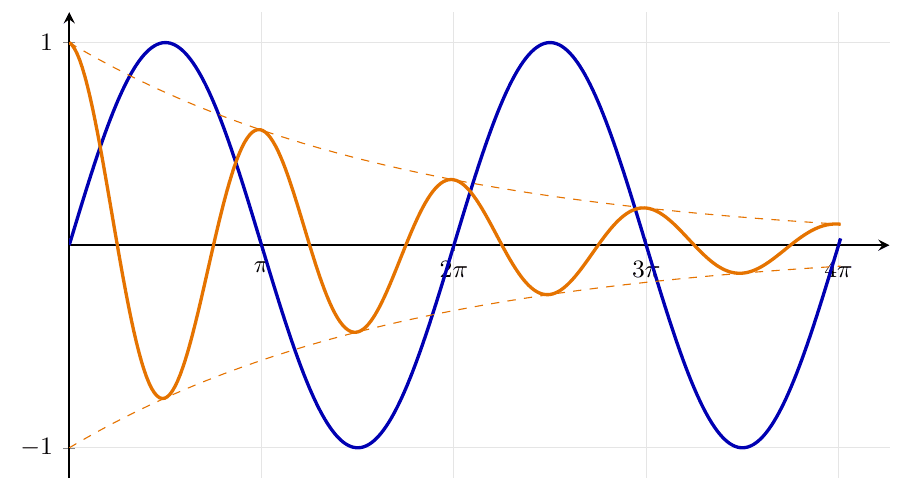
\includegraphics[width=0.9\linewidth]{images/curves.png}
    \end{tikzfigure}
    \vspace{1em}
    \begin{center}
      \begin{tabular}{lcc}
        \toprule
        Trial & $\lambda$ & Error (\%) \\
        \midrule
        1 & 0.182 & 1.1 \\
        2 & 0.179 & 0.6 \\
        \bottomrule
      \end{tabular}
    \end{center}
  }

  \block{Discussion}{
    The discussion compares the results with earlier work and sets out
    their limits.
  }

  \block{Conclusion}{
    The conclusion recalls the main message in one or two sentences.
  }
\end{columns}

\block{References}{
  \small
  D.~E. Knuth, \emph{The \TeX book}, Addison-Wesley, 1984.
}

\end{document}
